% {\bf A compulsory chapter,     of roughly $10$ pages} 
% \vspace{1cm} 

% \noindent
% This chapter is intended to describe the technical basis on which execution
% of the project depends.  The goal is to provide a detailed explanation of
% the specific problem at hand, and existing work that is relevant (e.g., an
% existing algorithm that you use, alternative solutions proposed, supporting
% technologies).  

% Per the same advice in the handbook, note there is a subtly difference from
% this and a full-blown literature review (or survey).  The latter might try
% to capture and organise (e.g., categorise somehow) {\em all} related work,
% potentially offering meta-analysis, whereas here the goal is simple to
% ensure the dissertation is self-contained.  Put another way, after reading 
% this chapter a non-expert reader should have obtained enough background to 
% understand what {\em you} have done (by reading subsequent sections), then 
% accurately assess your work.  You might view an additional goal as giving 
% the reader confidence that you are able to absorb, understand and clearly 
% communicate highly technical material.

As outlined in Chapter \ref{chap:context}, the objective of this project is to use deep learning to automate the calculation of the amount of skeletal matter produced by corals annually. This chapter introduces and briefly describes the techniques used in order to achieve this goal.

\section{Deep Learning}
\label{sec:deeplearning}

Based loosely on the structure of the brain, artificial neural networks (ANNs) are computational models that have proved useful in a wide range of applications~\cite{lecun2015deep, healthcare, nlp}\textemdash a notable example being the recent success of convolutional neural networks in the field of computer vision~\cite{compvision, semanticsegreview}. Deep learning is a form of machine learning that concerns the use of ANNs with many layers\textemdash hence the name ``deep'' learning. The field has seen a significant increase in popularity in recent years since a network named AlexNet famously won the ImageNet Large Scale Visual Recognition Challenge in 2012\footnote{\url{http://www.image-net.org/challenges/LSVRC/2012/results.html}}, performing considerably better than the previous state-of-the-art~\cite{alexnet}.

A typical fully connected ANN is a layered network of ``neurons'' connected by a series of ``weights''. A neuron is simply an object that produces a weighted sum of some number of inputs. This weighted sum is often passed through a non-linear ``activation'' function and the final result is referred to as the ``activation'' of the neuron. When values are supplied to the input neurons of the network, these values are forward-propagated through the network, activating each layer of neurons which, in turn, activate the next layer. The resulting activations of the neurons in the final layer are the output of the network.

\subsection{Convolutional Neural Networks}

The convolutional neural network (CNN) is a type of neural network named after the discrete convolution operation that sets these models apart from typical fully connected ANNs. The convolution operation makes use of surrounding pixels in order to change the value of a central pixel. The 2D discrete convolution operation is defined as

\begin{equation}
    g(x,y)=\sum_{i=1}^{m}\sum_{j=1}^{n}f(x-j,y-k)h(j,k)
\end{equation}

\noindent
where $f$ is the input image, $h$ is an $m\times n$ kernel, and $g$ is the resulting image.

CNNs often contain multiple convolutional layers in which increasingly complex features of an image may be detected by making use of a combination of simpler features detected in previous layers. A convolutional layer convolves the channels of an image with multiple learned kernels. A channel is simply a component of an image\textemdash an RGB image, for example, consists of three channels, whilst a greyscale image consists of only one. The output of these operations will be multiple modified images that are referred to as ``feature maps''. These feature maps can then be used as the input channels to the next layer, and so on.

As well as the convolution operation, the max-pooling operation is often used. The max-pooling operation is used to decrease the dimensionality of the input in attempt to force the network to ``learn'' features present in the input. These operations are illustrated in Figure \ref{fig:operations}.

\begin{figure}[t]
    \centering
    \begin{subfigure}[t]{0.43\textwidth}
        \centering
        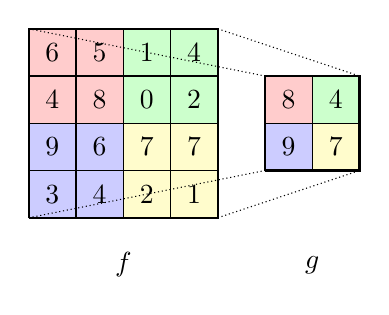
\begin{tikzpicture}[scale=0.6]
    \filldraw[color=blue, opacity=0.2] (0,0) rectangle (2,2);
    \filldraw[color=red, opacity=0.2] (0,2) rectangle (2,4);
    \filldraw[color=green, opacity=0.2] (2,2) rectangle (4,4);
    \filldraw[color=yellow, opacity=0.2] (2,0) rectangle (4,2);

    \filldraw[color=blue, opacity=0.2] (5,1) rectangle (6,2);
    \filldraw[color=red, opacity=0.2] (5,2) rectangle (6,3);
    \filldraw[color=green, opacity=0.2] (6,2) rectangle (7,3);
    \filldraw[color=yellow, opacity=0.2] (6,1) rectangle (7,2);

	\draw [thick] (0,0) -- (0,4) -- (4,4) -- (4,0) -- (0,0);
    \draw (0,1) -- (4,1);
    \draw (0,2) -- (4,2);
    \draw (0,3) -- (4,3);
    \draw (1,0) -- (1,4);
    \draw (2,0) -- (2,4);
    \draw (3,0) -- (3,4);
    \node at (0.5, 0.5) {3};
    \node at (1.5, 0.5) {4};
    \node at (2.5, 0.5) {2};
    \node at (3.5, 0.5) {1};
    \node at (0.5, 1.5) {9};
    \node at (1.5, 1.5) {6};
    \node at (2.5, 1.5) {7};
    \node at (3.5, 1.5) {7};
    \node at (0.5, 2.5) {4};
    \node at (1.5, 2.5) {8};
    \node at (2.5, 2.5) {0};
    \node at (3.5, 2.5) {2};
    \node at (0.5, 3.5) {6};
    \node at (1.5, 3.5) {5};
    \node at (2.5, 3.5) {1};
    \node at (3.5, 3.5) {4};
    
    \draw[densely dotted] (0,0) -- (5,1);
    \draw[densely dotted] (0,4) -- (5,3);
    \draw[densely dotted] (4,4) -- (7,3);
    \draw[densely dotted] (4,0) -- (7,1);
    
    \draw [thick] (5,1) -- (5,3) -- (7,3) -- (7,1) -- (5,1);
    \draw (6,1) -- (6,3);
    \draw (5,2) -- (7,2);
    
    \node at (5.5, 1.5) {9};
    \node at (6.5, 1.5) {7};
    \node at (5.5, 2.5) {8};
    \node at (6.5, 2.5) {4};
    
    \node at (2, -1) {$f$};
    \node at (6, -1) {$g$};
\end{tikzpicture}
    \vspace*{1mm}
    \caption{2D Max-pooling}
    \end{subfigure}
    ~
    \begin{subfigure}[t]{0.55\textwidth}
        \centering
        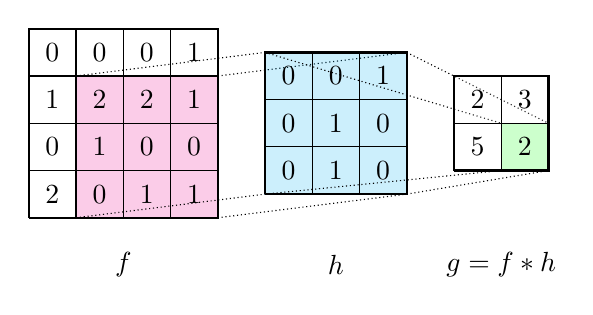
\begin{tikzpicture}[scale=0.6]
    \filldraw[color=magenta, opacity=0.2] (1,0) rectangle (4,3);

	\draw [thick] (0,0) -- (0,4) -- (4,4) -- (4,0) -- (0,0);
    \draw (0,1) -- (4,1);
    \draw (0,2) -- (4,2);
    \draw (0,3) -- (4,3);
    \draw (1,0) -- (1,4);
    \draw (2,0) -- (2,4);
    \draw (3,0) -- (3,4);
    
    \node at (0.5, 0.5) {2};
    \node at (1.5, 0.5) {0};
    \node at (2.5, 0.5) {1};
    \node at (3.5, 0.5) {1};
    \node at (0.5, 1.5) {0};
    \node at (1.5, 1.5) {1};
    \node at (2.5, 1.5) {0};
    \node at (3.5, 1.5) {0};
    \node at (0.5, 2.5) {1};
    \node at (1.5, 2.5) {2};
    \node at (2.5, 2.5) {2};
    \node at (3.5, 2.5) {1};
    \node at (0.5, 3.5) {0};
    \node at (1.5, 3.5) {0};
    \node at (2.5, 3.5) {0};
    \node at (3.5, 3.5) {1};
    
    \draw[densely dotted] (1,0) -- (5,0.5);
    \draw[densely dotted] (1,3) -- (5,3.5);
    \draw[densely dotted] (4,3) -- (8,3.5);
    \draw[densely dotted] (4,0) -- (8,0.5);
    
    \filldraw[color=cyan, opacity=0.2] (5,0.5) rectangle (8,3.5);
    
    \draw [thick] (5,0.5) -- (5,3.5) -- (8,3.5) -- (8,0.5) -- (5,0.5);
    \draw (5,2.5) -- (8,2.5);
    \draw (5,1.5) -- (8,1.5);
    \draw (6,0.5) -- (6,3.5);
    \draw (7,0.5) -- (7,3.5);
    
    \node at (5.5, 1) {0};
    \node at (6.5, 1) {1};
    \node at (7.5, 1) {0};
    \node at (5.5, 2) {0};
    \node at (6.5, 2) {1};
    \node at (7.5, 2) {0};
    \node at (5.5, 3) {0};
    \node at (6.5, 3) {0};
    \node at (7.5, 3) {1};
    
    \draw[densely dotted] (5,0.5) -- (10, 1);
    \draw[densely dotted] (5,3.5) -- (10, 2);
    \draw[densely dotted] (8,3.5) -- (11, 2);
    \draw[densely dotted] (8,0.5) -- (11, 1);
    
    \filldraw[color=white, opacity=0.2] (9,1) rectangle (10,2);
    \filldraw[color=white, opacity=0.2] (9,2) rectangle (10,3);
    \filldraw[color=green, opacity=0.2] (10,1) rectangle (11,2);
    \filldraw[color=white, opacity=0.2] (10,2) rectangle (11,3);
    
    \draw [thick] (9,1) -- (9,3) -- (11,3) -- (11,1) -- (9,1);
    \draw (10,1) -- (10,3);
    \draw (9,2) -- (11,2);
    
    \node at (9.5, 1.5) {5};
    \node at (10.5, 1.5) {2};
    \node at (9.5, 2.5) {2};
    \node at (10.5, 2.5) {3};
    
    \node at (2, -1) {$f$};
    \node at (6.5, -1) {$h$};
    \node at (10, -1) {$g=f\ast h$};
\end{tikzpicture}
        \vspace*{1mm}
        \caption{2D Convolution}
    \end{subfigure}
    \caption{Illustrations of the 2D max-pooling and convolution operations. \textbf{(a)} The max-pooling operation shown takes an input image $f$ and uses a $2\times 2$ filter and stride of two to produce the output image $g$. Note that the maximum value in each coloured region of the input is the resulting value of the corresponding regions of the output. \textbf{(b)} The convolution operation shown takes an input image $f$ and uses a $3\times 3$ kernel $h$ with a stride of one to produce the output image $g=f\ast h$, where $\ast$ denotes the convolution operation. Note that the kernel shown in the convolution operation is ``flipped'' in both the $x$ and $y$ axes before the element-wise multiplication and summation takes place.}
    \label{fig:operations}
\end{figure}

Another feature of CNNs that set them apart from their fully connected counterparts is the localised ``receptive fields'' of the neurons present in convolutional layers. Whilst neurons present in a fully connected layer can receive input from every neuron in the previous layer, neurons present in a convolutional layer can only receive input from a small amount of neighbouring neurons in the previous layer. For example, if a $3\times 3$ kernel is used, a neuron's activation can only be influenced by nine neurons in the previous layer. This area of input that can influence a neuron is called its receptive field. This is one of the reasons why during hyper parameter optimisation, kernel sizes from various layers may be tuned in order to increase or decrease the size of neurons' receptive fields. Hyper parameter optimisation is discussed in Section \ref{sec:hyperparam}.

\subsection{Backpropagation}
\label{sec:backprop}

First popularised by Rumelhart et al. in 1986~\cite{rumelhart}, the backpropagation algorithm is still the main learning mechanism used in neural networks today. Once a loss function is defined to measure the performance of the network, backpropagation can be used to compute the derivative of the loss function with respect to each weight in the network using the chain rule. The derivatives are calculated one layer at a time, iterating backward from the output layer. Since the backpropagation algorithm makes use of the chain rule, the loss function must be differentiable. This must also be the case for the chosen activation functions for each neuron.

An optimisation algorithm can then use these computed derivatives to adjust each weight in order to minimise the chosen loss function. Loss functions used throughout this project are discussed in Section \ref{sec:loss}.

\subsection{Optimisation Algorithms}

Once the derivatives\textemdash or ``gradients''\textemdash have been calculated, an optimisation algorithm is used to determine the exact value each weight should be updated to. When training deep neural networks, some variant of the gradient descent algorithm is often used. Gradient descent~\cite[p. 536]{gradient} is an iterative algorithm designed to find local minima of some differentiable function\textemdash in this case, the loss function. A visualisation of the gradient descent algorithm is shown in Figure \ref{fig:gd}. The gradient descent algorithm evaluates the loss function over the entire dataset before taking a ``step'' in the direction of the gradient computed. A step consists of updating the value of every weight in order to decrease the average loss value that would be achieved by the network when processing the dataset. Evaluating the loss function over the entire dataset once is referred to as an ``epoch''.

The size of the weight update is not only determined by the gradient calculated, but also by a hyper parameter called the ``learning rate''. For example, gradient descent calculates the update for a single weight $w$ as

\begin{equation}
    w := w - \eta\nabla\ell(w)
\end{equation}

\noindent
where $\eta$ is the learning rate and $\nabla\ell(w)$ is the derivative of the loss function $\ell$ with respect to $w$. Choosing an appropriate learning rate is challenging but is essential to allow an optimisation algorithm to converge to a local minimum. A learning rate that is too large can cause the loss function to fluctuate around the minimum, impeding convergence or even causing divergence. The learning rate hyper parameter has a significant effect on training and is one of the most important parameters tuned in the hyper parameter optimisation process (see Section \ref{sec:hyperparam}).


\subsubsection{Stochastic Gradient Descent}

Issues arise when using gradient descent with larger datasets, as evaluating the loss function over the entire dataset before a step can be taken becomes increasingly computationally costly~\cite{gdbad}. These issues have given rise to the popularity of the stochastic gradient descent (SGD) and the mini-batch gradient descent optimisation algorithms. SGD is a variant of the gradient descent algorithm that takes a step each time a sample is processed rather than only once the entire dataset is processed. Mini-batch gradient descent is yet another variant of gradient descent in which weights are updated after evaluating the loss function over a subset\textemdash or ``batch''\textemdash of the training samples.

\begin{figure}[t]
    \centering
    \begin{tikzpicture}[scale=1.1]
	\begin{axis}[
% 	colormap/greenyellow,
	colormap name=cool2,
% 	view={0}{90}
	xlabel=$x$,
	ylabel=$y$,
	zlabel=Loss,
	zmin=0.1, zmax=1.9,
	xtick distance=175,
	ytick distance=175,
	xticklabels=\empty,
	yticklabels=\empty,
	zticklabels=\empty
	]
% 	\addplot3[surf,
% 		domain=0:360,samples=40] 
% 		{0.5*sin(x-100)*sin(y-50) - 0.000005*((x-100)^2) + 0.000005*((y-50)^2) + 1};
    \addplot3 [surf, mesh/rows=36] table [x=xs, y=ys, z=zs, col sep=comma] {csv/surf.csv};
    
	\addplot3 [black, mark=*, line width=0.8pt, mark size=0.8pt] table [x=xs, y=ys, z=zs, col sep=comma] {csv/sgd.csv};
	
	\addplot3 [black, mark=*, line width=0.8pt, mark size=0.8pt] table [x=xs, y=ys, z=zs, col sep=comma] {csv/sgd3.csv};
	
	\node[] at (axis cs: 320, 200, 1.9) {\scriptsize{($x_0, y_0, \ell(x_0, y_0)$)}};
	
	\node[] at (axis cs: 260, 200, 0.1) {\scriptsize{($x_n, y_n, \ell(x_n, y_n)$)}};
	\end{axis}
\end{tikzpicture}
    \caption{A diagram visualising the gradient descent algorithm for a model containing two trainable parameters, $x$ and $y$. Given a random starting configuration with parameters $x_0$ and $y_0$, the average loss value that would be achieved when processing the entire dataset is given by $\ell(x_0, y_0)$. Say gradient descent takes $n$ steps in the direction of steepest descent at each iteration until the loss value converges to some local minimum, $x_n$ and $y_n$ would be the final parameter values and the final loss would be $\ell(x_n, y_n)$. It is worth noting that even though the two starting configurations shown in the diagram both converge to the same local minimum, this might not always be the case. A starting configuration nearer to one of the other possible local minima would most likely not converge to the example local minimum $\ell(x_n, y_n)$ shown.}
    \label{fig:gd}
\end{figure}

\subsubsection{Adam}

First introduced by Kingma and Ba in 2014, Adam~\cite{adam} is an optimisation algorithm that is also based off of SGD. However, rather than using the same learning rate across all parameters, Adam computes individual adaptive learning rates for different parameters. These individual learning rates are based off of estimates of the first moment (the mean) and second moment (the uncentered variance) of the gradients~\cite{gdbad}. Kingma and Ba showed empirically that Adam works well in practice and compares favourably to other optimisation algorithms when optimising both fully connected ANNs and deep CNNs.

\subsection{Loss functions}
\label{sec:loss}

A loss function takes both the actual and predicted values of a training sample, and outputs some measure of how well a model performed by producing that prediction. As mentioned in Section \ref{sec:backprop}, backpropagation makes use of the derivative of the loss function with respect to each parameter in order to minimise the loss achieved. If the appropriate loss function is chosen, minimising the loss should improve the performance achieved by the network. It is for this reason that loss functions must be differentiable. The loss functions that were experimented with throughout this project are outlined below.

\subsubsection{Binary Cross-Entropy Loss}

\begin{equation}
    L(y, \hat{y})=-\frac{1}{N} \sum_{i=0}^{N}\left(y * \log \left(\hat{y}_{i}\right)+(1-y) * \log \left(1-\hat{y}_{i}\right)\right)
\end{equation}

where $y$ is the actual value, and $\hat{y}$ is the predicted value.

\subsubsection{Focal Loss}

\begin{equation}
    \mathrm{FL}\left(p_{\mathrm{t}}\right)=-\left(1-p_{\mathrm{t}}\right)^{\gamma} \log \left(p_{\mathrm{t}}\right)
\end{equation}

~\cite{focalloss}

\subsubsection{Dice coefficient}

\subsection{Accuracy Metrics}

Although loss functions can be used to measure performance, their main purpose is to be used to train the network. To quantify the performance achieved by a network, an accuracy metric should instead be used. Accuracy metrics do not play a direct role in training networks, though they can be used indirectly\textemdash for example, to determine whether or not to continue training. Choosing an appropriate accuracy metric is essential and proved challenging throughout this project. The main accuracy metric decided upon was based off of the Hausdorff distance discussed in Section \ref{sec:hausdorff}.

\subsection{Datasets}

Introduce train test val split and what they are all used for.

Referred to as a ``beautiful free lunch'' by Geoffrey Hinton~\cite[p. 141]{earlystopping}, early stopping is.

\subsection{Pooling}

\subsection{Overfitting}

The term overfitting is used to describe when a model performs well on the data on which it is trained, yet poorly on data which it has not yet been exposed to.

\subsubsection{Data augmentation}

Data augmentation is the process of augmenting the labelled training data in some way in order to increase the amount of training data available. This augmentation can be performed ``online'' with each training sample being randomly augmented during the training process, or it can be performed ``offline'' with the augmentation taking place before training. The training data can be augmented in many ways. Common examples for 2D images are: random rotations within some predefined range, random changes to brightness levels, and random horizontal and vertical flips. Data augmentation is used to reduce overfitting.

\subsubsection{Dropout}

Another technique often used to reduce overfitting, is ``dropout''.

\subsection{Hyper parameter optimisation}
\label{sec:hyperparam}

Define what a parameter and hyper parameter is. Talk about diff algorithms (genetic vs brute force).

\subsection{SegNet}

Mention that segnet and unet are both fully convolutional so no dense layers (fully connected)

\subsection{U-Net}

Presented by Ronneberger et al. in 2015~\cite{ronneberger2015u}, U-Net is a convolutional neural network architecture that was initially used to perform instance segmentation on biomedical images, but has since been used on a wider range of visual data. The U-Net architecture consists of three sections: the contracting path, the bottleneck, and the expanding path. The contracting path follows the typical architecture of a convolutional network, in that the image is gradually downsampled and the number of feature channels is increased. The expansion path then gradually reconstructs the image via `up-convolutions'. Throughout the expansion path, the feature channels from the corresponding contraction layers are appended to the feature channels in the expansion layers. This allows the features that are learned whilst contracting the image to also be used to reconstruct it. A diagram of the U-Net architecture is shown in Figure~\ref{fig:unet}.

\begin{figure}[t]
    \centering
    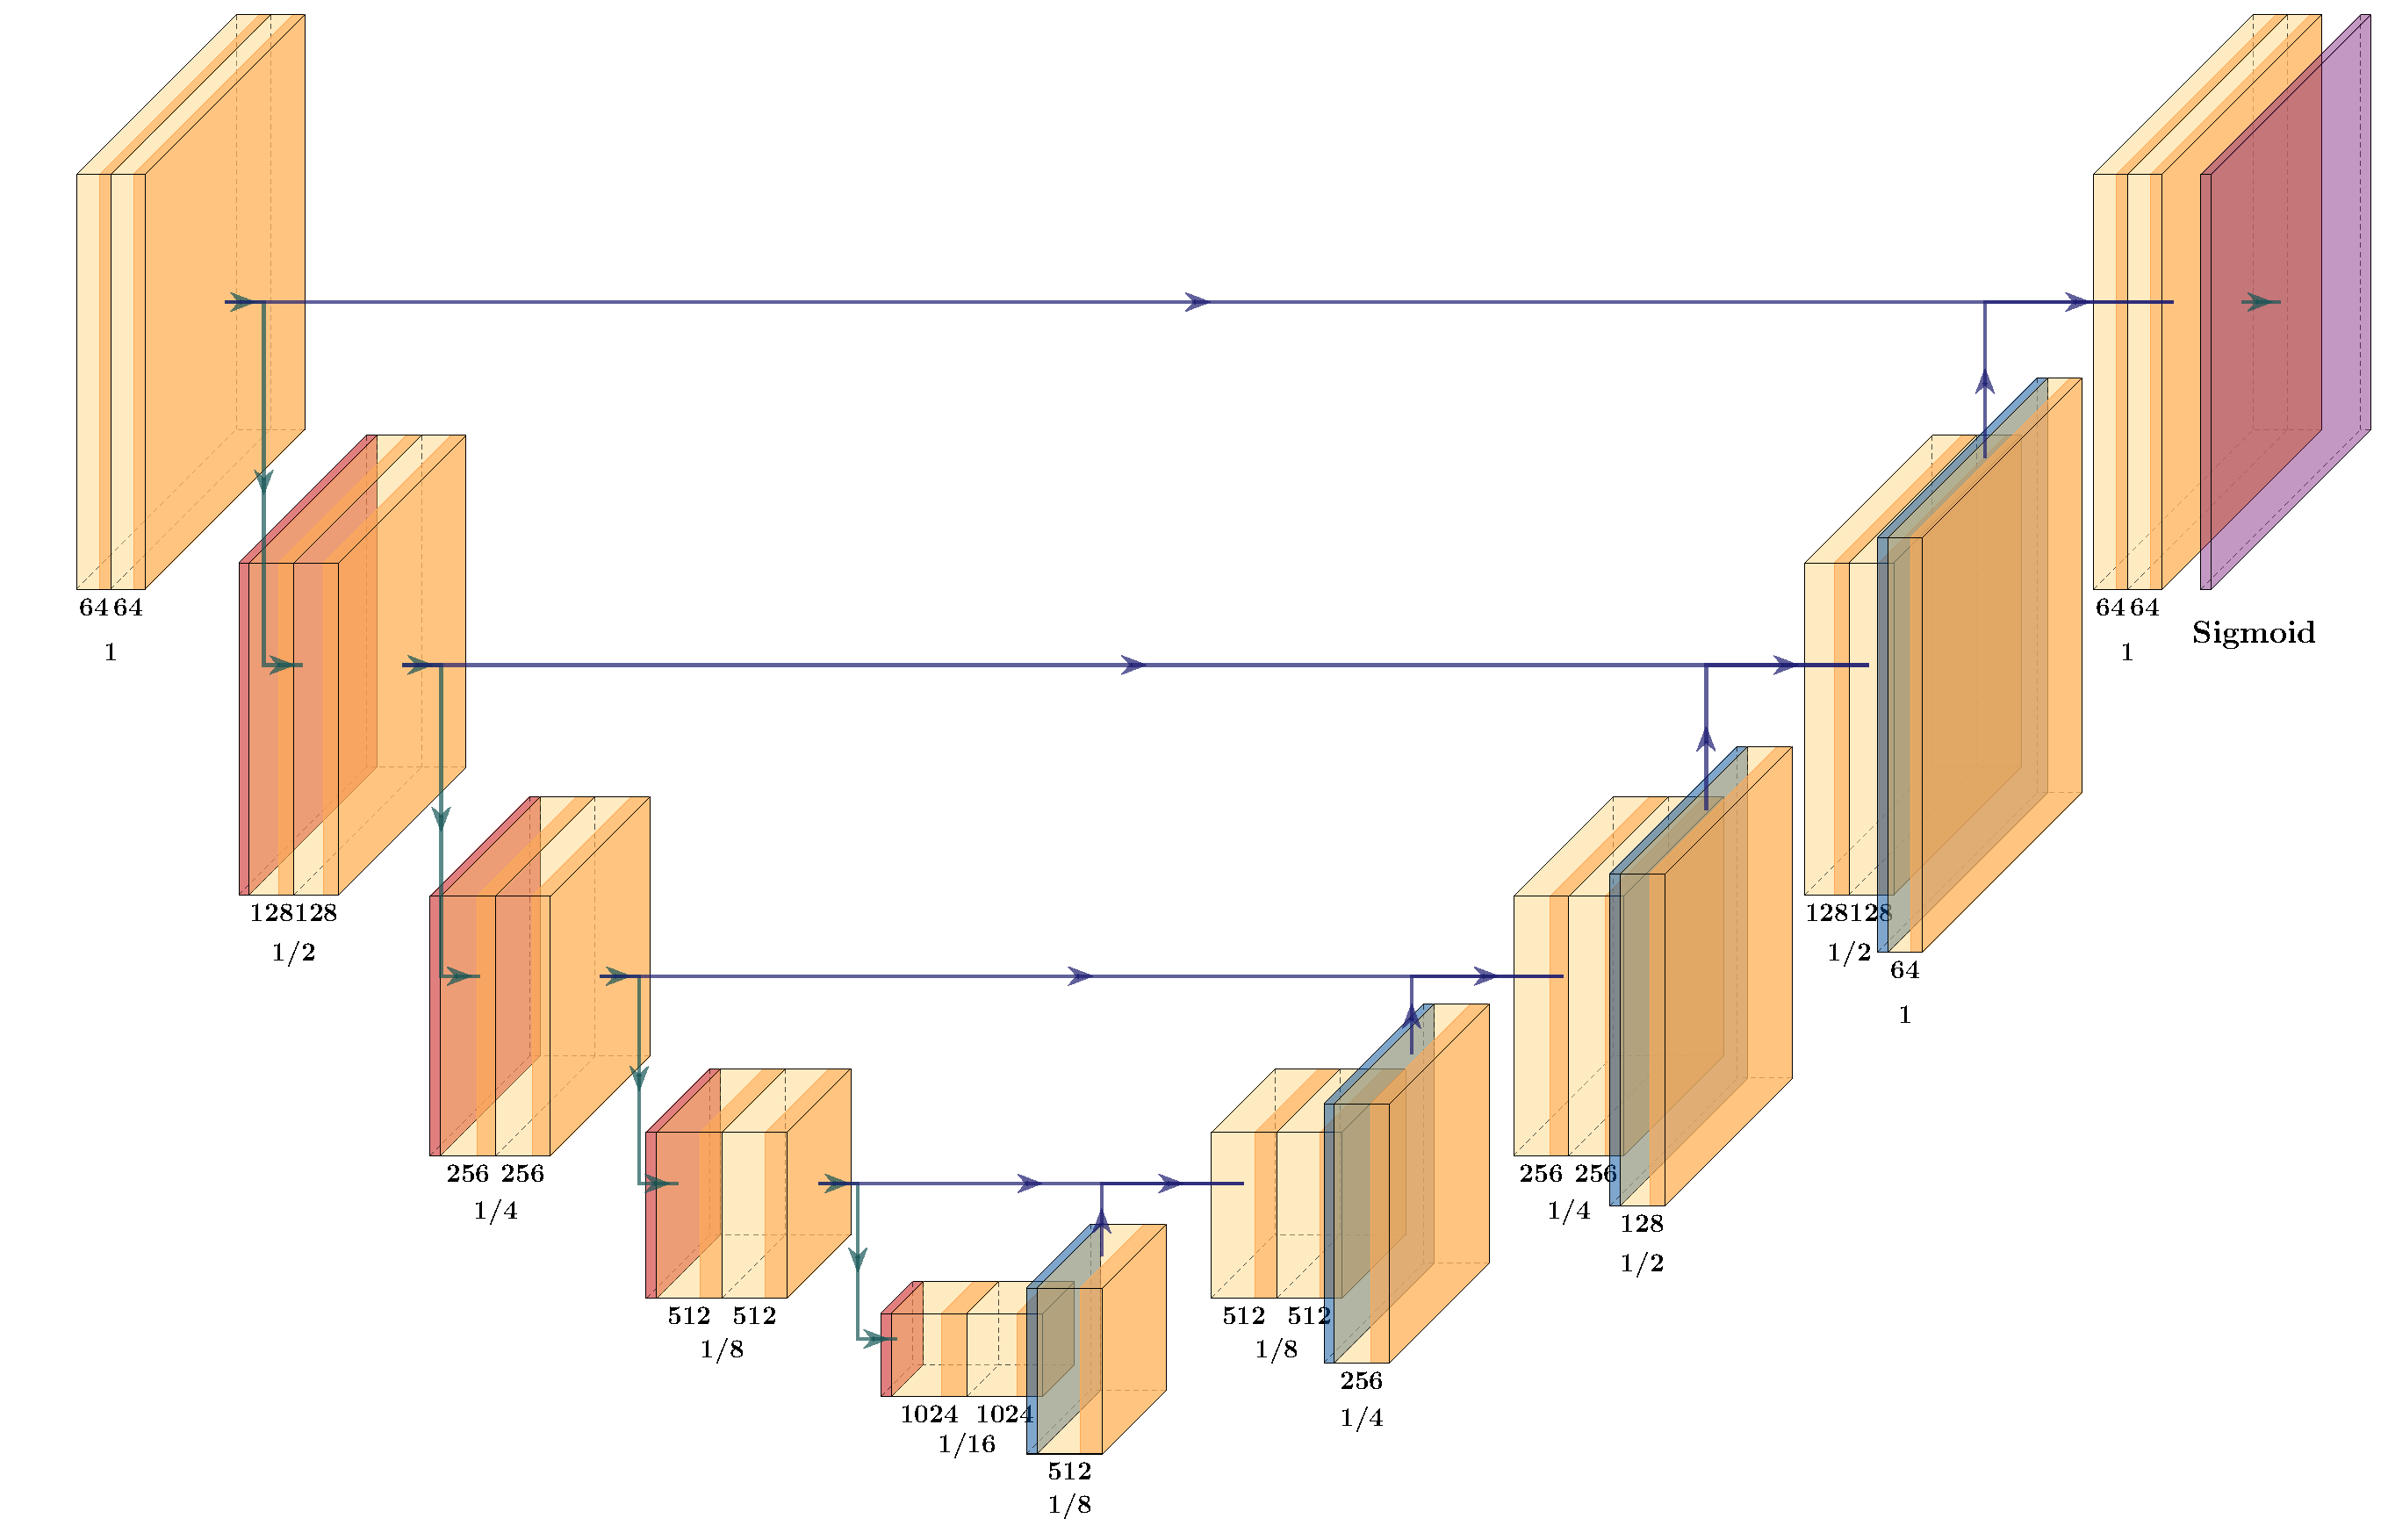
\includegraphics[width=1\textwidth]{images/U-Net.pdf}
    \caption{A diagram of the U-Net architecture. Each cube represents a layer. The orange cubes represent convolutional layers, the red cubes represent max-pooling, and the blue cubes represent up-convolutions. The green arrows represent the feedforward of information from one layer to the next, whereas the blue arrows represent the concatenation of the feature maps of one layer to another.}
    \label{fig:unet}
\end{figure}

\subsection{CycleGANs and pix2pix}

Throughout this project, various deep learning techniques are utilised in an attempt to maximise the performance achieved.

\section{Classical Image Processing Techniques}

\subsection{Hausdorff distance}
\label{sec:hausdorff}

\section{Supporting Technologies}

\subsection{Keras}